\section{Introduction}
Additive manufacturing in general

FDM is

FDM is used for...

FDM works by depositing beads in flat layers

Outer walls are contour following because the resolution determined by the bead width is worse than the spatial accuracy of the XYZ positioning system.

Naive method

mechanical properties of FDM parts and relations with bead width




\subsection{Problem}
Thin model parts either produce overfill or underfill in the naive method.

3D models may have parts with pieces with a thickness of non-integer multiples of the nominal bead width.
How can we fill such a shape?
We must employ varying line width.

Too thin lines cannot be fabricated accurately. 
See \cref{extremal_bead_widths}.

\begin{figure}
\centering
\setlength{\figwidth}{.4\columnwidth}
%\begin{subfigure}{\figwidth}\centering
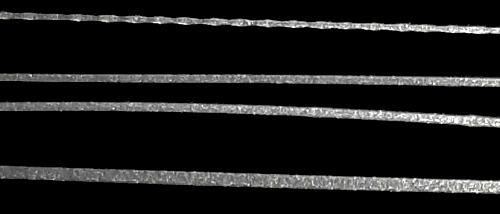
\includegraphics[width=\columnwidth]{sources/intro/thin_extrusion.jpg}
%\caption{Thin}
%\end{subfigure}
\caption{
Extremal bead widths.
Bead widths from top to bottom: \SI{0.2}{\milli\meter}, \SI{0.3}{\milli\meter}, \SI{0.4}{\milli\meter}, \SI{0.5}{\milli\meter}.
Too thin lines cannot be manufactured reliably.
}
\label{extremal_bead_widths}
\end{figure}



\subsection{Significance}

There is a large body of literature on relating process parameters such as bead width to various mechanical properties of the end part.
In order to accurately fabricate something with prescribed mechanical properties we need to print while employing roughly homogenous line width.

Line width is influenced by the following factors:
\begin{itemize}
\item Larger for filling cravices
\item Larger or smaller (?) for heat dissipation
\item Larger for larger contact surface, so better adhesion \cite{N.Turner2014}
\item Larger fills up an area faster \cite{ahn2002anisotropic}
\item Smaller for better quality top surfaces \cite{ahn2002anisotropic}
\item Smaller for overhangs
\item Smaller to compensate for die swell
\item Smaller for more detail, less rounded corners \cite{N.Turner2014}
\end{itemize}



\iffalse

``Small bead width increases build time. Small bead width increases surfacequality.''\cite{ahn2002anisotropic}

``The final width of the road determines the resolution that can be achieved in the print process, as well as the contactarea between neighboring beads.  The rounded, oblong shape of  the  bead  inevitably  leads  to  small  voids  in  the  part.  The strength   of   the   bond   between   neighboring   roads,   and ultimately the overall mechanical properties of the part, will depend on the contact area between those beads and the size of the voids.''\cite{N.Turner2014}
\fi



\subsection{Goal}
\begin{itemize}
\item Accurate fabrication of thin walls
\item Prevent underfilling and overfilling
\item ... for accurately matching stiffness properties
\item ... and/or translucency properties
\item Without generating paths smaller than \SI{70}{\percent} of the nozzle size
\item While generating maximally paths of \SI{140}{\percent} of the nozzle size
\end{itemize}



\subsection{Contributions}
\begin{itemize}
\item A framework for generating conentric toolpaths with variable width
\end{itemize}

This work is patent pending, but the source code is available open source.

